\newpage
\section{Información para entregar}\label{sec:Info}

Una vez realizado el cálculo y consolidados los resultados, se debe presentar para su aprobación una memoria de cálculo completa que recoja el detalle de los pasos realizados, de la información relevada del plano y de las suposiciones asumidas. Esta memoria de cálculo debe permitir al lector reconstruir por su propia cuenta el procedimiento llevado a cabo.

Esta memoria de cálculo debe contener, como mínimo, la siguiente información:

\begin{enumerate}
    
    \item Densidad \textit{normal} y densidad \textit{estándar} del gas natural quemado en la caldera.
    
    \item $PCI$\footnote{Poder calorífico inferior, o $LHV$ según sus siglas en inglés (lower heating value). Definimos al $PCI$ como el calor liberado por la combustión completa y estequiométrica del combustible con productos y reactivos en condiciones \textit{estándar}. A este calor se le debe restar el calor de vaporización del agua a la temperatura \textit{estándar}.} del gas natural quemado en la caldera. Utilizar el script incluido \href{https://www.unitrove.com/engineering/tools/gas/natural-gas-calorific-value}{aquí}. Expresarlo en $\SI{}{\frac{kcal}{m^3S}}$, $\SI{}{\frac{kcal}{m^3N}}$ y en $\SI{}{\frac{kJ}{kg}}$.
    
    \item Caudal de gas natural quemado en la caldera, adoptando como válido el rendimiento térmico informado por el fabricante.
    
    \item Composición molar (o volumétrica) y másica de los gases de combustión en base húmeda. Masa molar de los gases de combustión. Caudal másico de los gases de combustión. Caudal volumétrico en condiciones \textit{normales} del aire de combustión. Relación gases húmedos-combustible para el exceso informado. Composición molar de los gases de combustión en base seca.
    
    \item Cuadro de temperatura de llama vs. emisividad de la llama. En él deben figurar el resultado para el valor dato, para este aumentado en un $15\%$ y para este disminuido en un $15\%$.
    
    \item Liberación de calor volumétrica y superficial del hogar.\footnote{La temperatura de llama es el único valor que se debe calcular tres veces, para distintas emisividades de llama. El resto de los valores, por ejemplo, las liberaciones de calor, solamente deben calcularse para la emisividad de llama dato.}
    
    \item Cuadro en el que figuren el coeficiente de intercambio térmico por radiación de los gases triatómicos, el coeficiente de transferencia por convección, el coeficiente de transferencia global, el área de transferencia y la diferencia de temperaturas media logarítmica para:
    \begin{itemize}
        \item Tubos pantalla,
        \item Sobrecalentador,
        \item Haz convectivo,
        \item Economizador.
    \end{itemize}
    
    \item Comparación del área necesaria para el sobrecalentamiento con el área dispuesta por el fabricante en el sobrecalentador.
    
    \item Cuadro resumen en el que figure el calor transferido en cada sector de la caldera, y el perfil térmico tanto de los gases húmedos como del agua-vapor (temperaturas a la entrada y salida de cada intercambio).
    
    \item Gráficos $T$ vs. $Q$ y $-1/T$ vs. $Q$. Utilizar como referencia los mostrados en las figuras \ref{im:TQ} y \ref{im:-1/TQ}.
    
    \item Temperatura de chimenea, calor cedido al ambiente en esta y rendimiento térmico obtenido de modo indirecto a partir de este calor. Comparación con el valor informado por el fabricante. Diferencia entre el consumo de combustible informado y el obtenido mediante este cálculo.
    
    \item Rendimiento exergético de la caldera, adoptando como válido el valor informado por el fabricante.
    
    \item Pinch point (y dónde se localiza) y approach point de la caldera.
    
    \item Conclusiones.

\end{enumerate}

\paragraph{Archivos de cálculo:}

En caso de que hayan sido usados scripts o programas, deben incluirse tanto los códigos como los archivos de cálculo. En caso de que sean archivos de \textit{EES}, estos deben entregarse convergiendo.

\paragraph{Unidades:}

En cuanto a unidades, se solicita expresar los caudales molares o volumétricos en $\SI{}{\frac{m^3N}{h}}$ o $\SI{}{\frac{m^3S}{h}}$ según el caso; las presiones del agua-vapor en $\SI{}{bar(g)}$; las temperaturas en $\SI{}{\celsius}$; y los caudales másicos en $\SI{}{\frac{kg}{h}}$. Estas son las unidades habituales en la que estos datos son expresados en la práctica.

\paragraph{Presentación de la información:} Se recomienda utilizar cuadros para presentar la información, ya que son muy cómodos para la lectura. Se desaconseja escribir los reemplazos en las fórmulas. Es suficiente incluir las expresiones, los valores asociados y los resultados obtenidos.


\begin{figure}[ht]
	\centerline{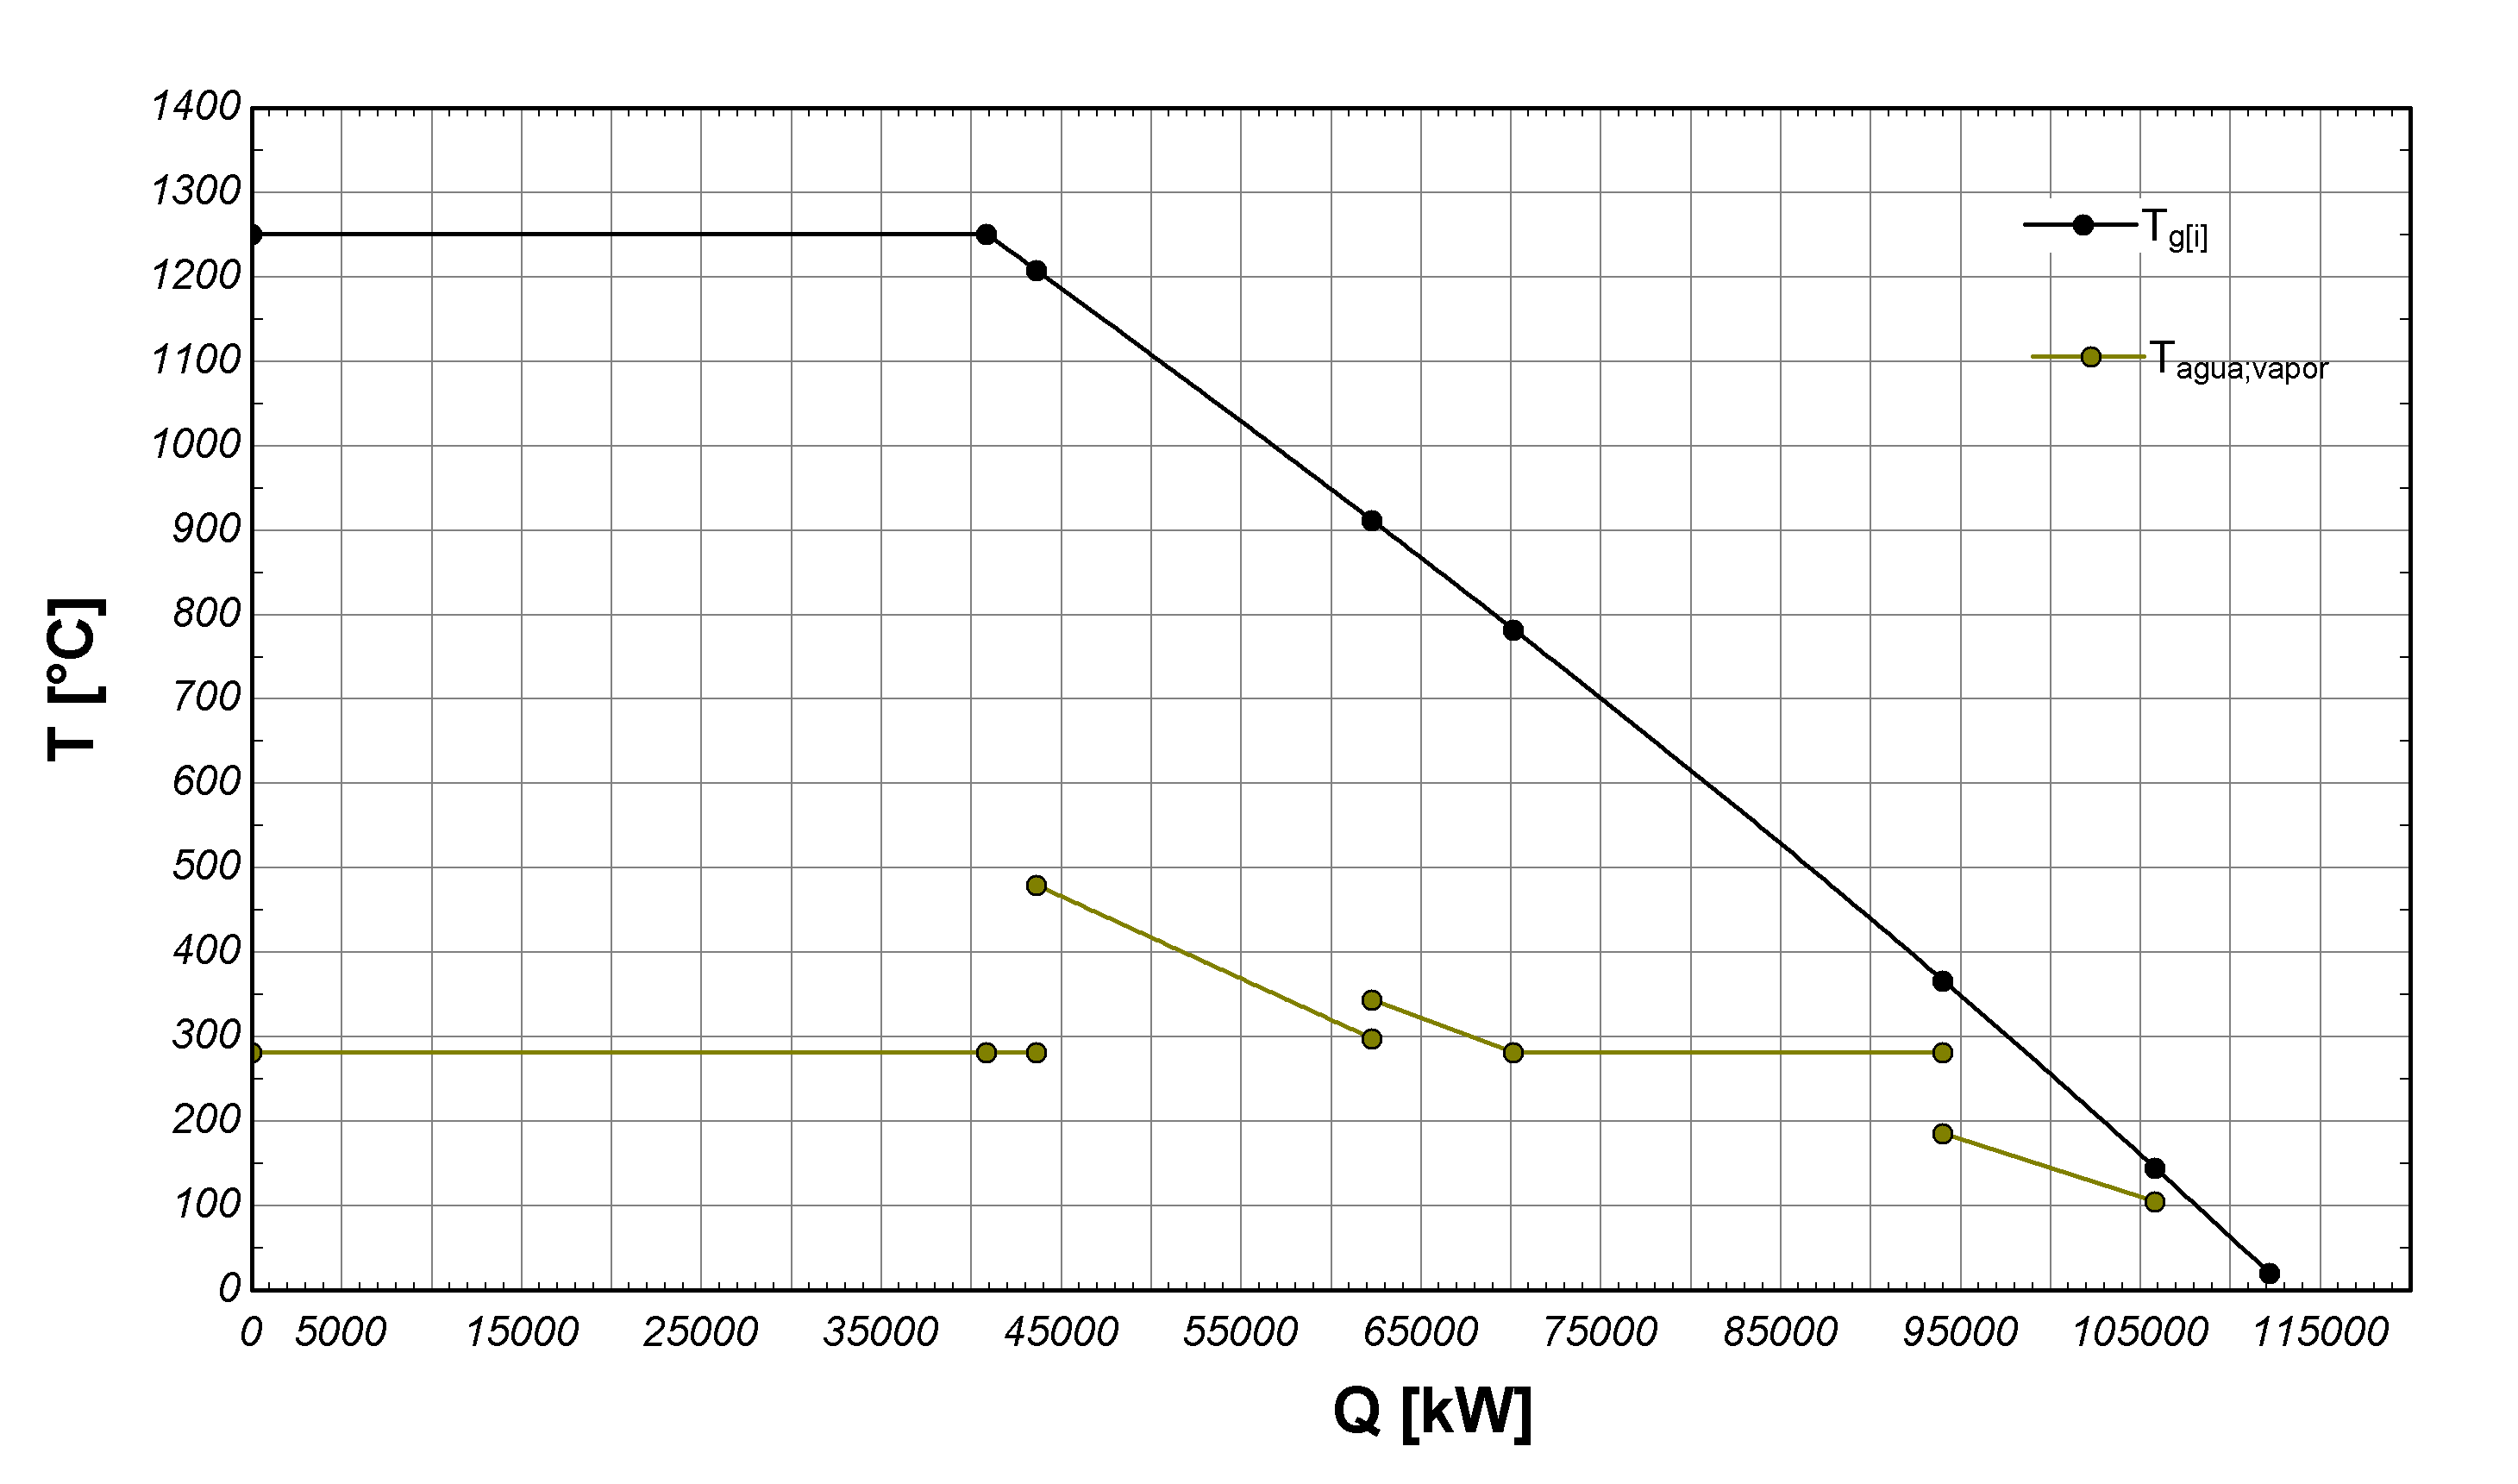
\includegraphics[scale=0.15]{graph_01.png}}
	\caption{\textit{En este caso la curva de la caldera es más compleja que la de este trabajo práctico, ya que el sobrecalentamiento está calculado en etapas, utilizando el área dispuesta por el fabricante, y la caldera tiene una atemperación de vapor intermedia.}}
	\label{im:TQ}
\end{figure}


\begin{figure}[ht]
	\centerline{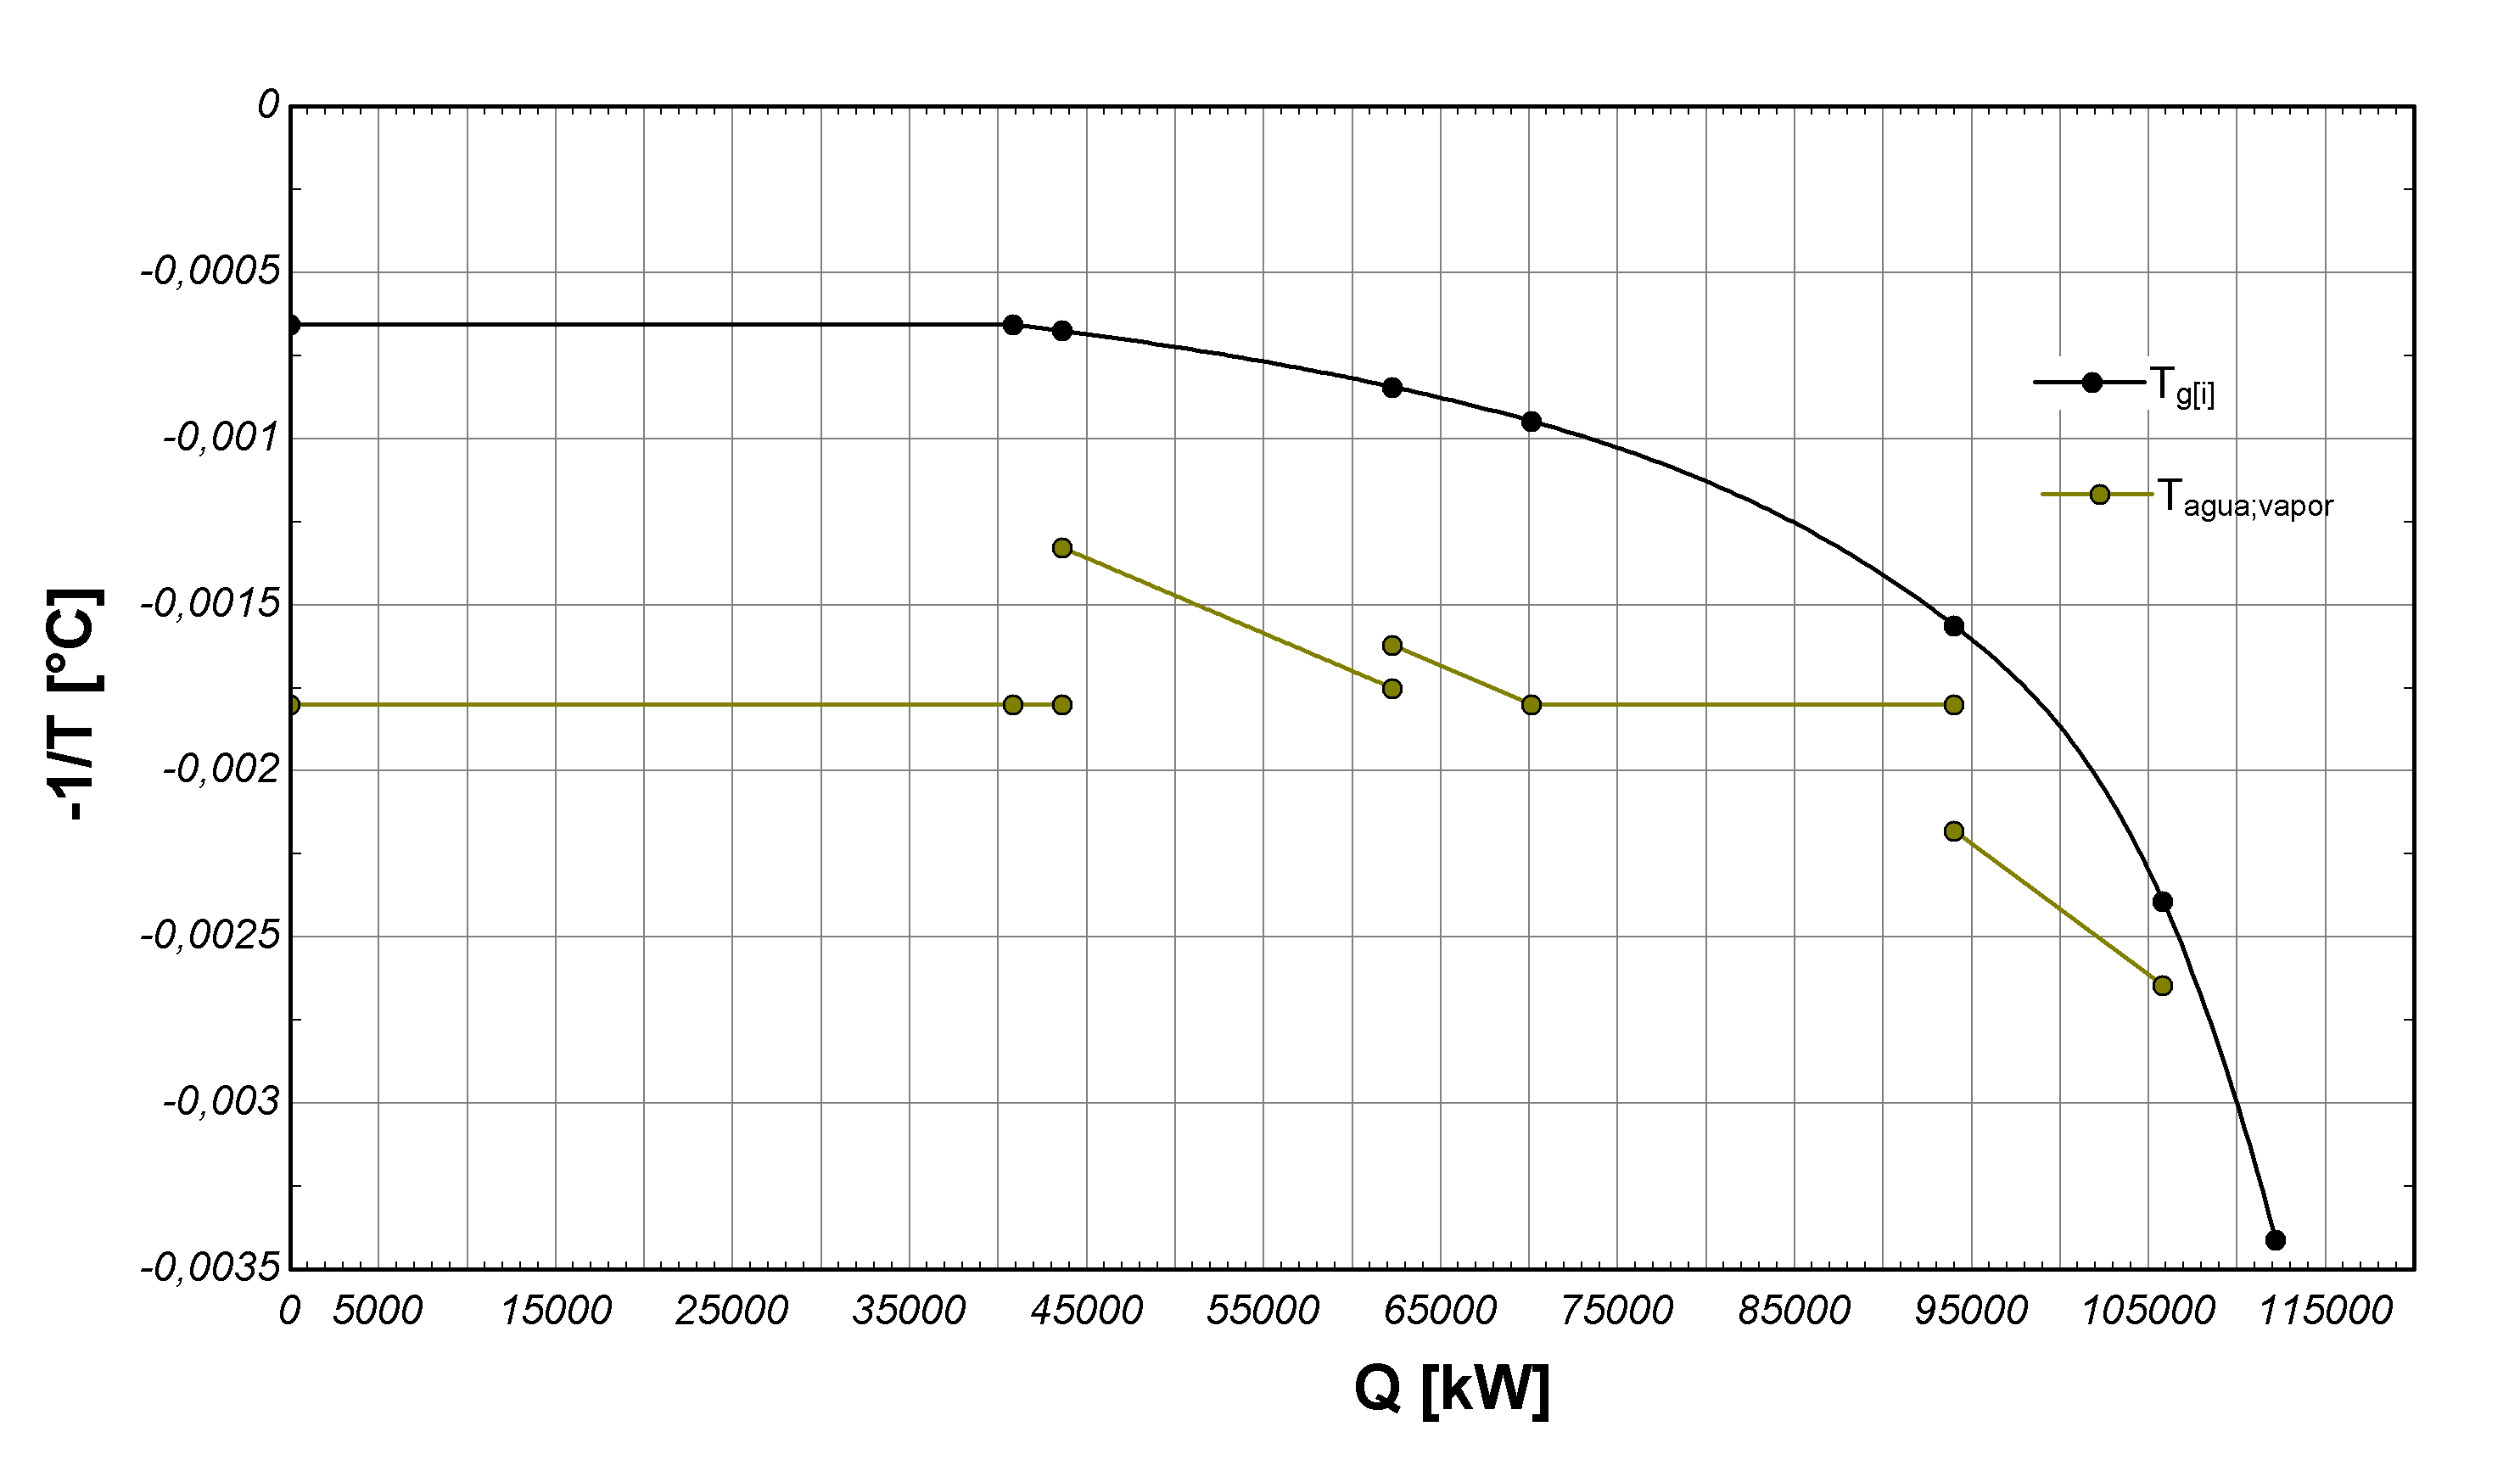
\includegraphics[scale=0.15]{graph_02.png}}
	\caption{\textit{En este caso la curva de la caldera es más compleja que la de este trabajo práctico, ya que el sobrecalentamiento está calculado en etapas, utilizando el área dispuesta por el fabricante, y la caldera tiene una atemperación de vapor intermedia.}}
	\label{im:-1/TQ}
\end{figure}


 




